%%%%%%%%%%%%%%%%%%%%%%%%%%%%%%%%%%%%%%%%%%%%%%%%%%%%%%%%%%%%%%%%%%%%%%%%%%
%
% StMcEvent - User Guide and Reference Manual -- LaTeX Source
%
% $Id: StMcEvent.tex,v 2.2 2000/02/03 23:04:30 calderon Exp $
%
% Authors:Michael A. Lisa
%         Thomas S. Ullrich
%         Manuel Calderon de la Barca Sanchez
%
%%%%%%%%%%%%%%%%%%%%%%%%%%%%%%%%%%%%%%%%%%%%%%%%%%%%%%%%%%%%%%%%%%%%%%%%%%
%
% Notes to the authors:
%
% - A template for a class reference is at the end of this file.
% - Wrap all names functions with \name{}
% - All code, examples, prototypes in \verb+ ... +\\
%   or \begin{verbatim} ... \end{verbatim}
% - Use \StMcEvent if you refer to the package itself (not the class)
%
% This file is best edit with xemacs and the 'Function' package loaded.
%
%%%%%%%%%%%%%%%%%%%%%%%%%%%%%%%%%%%%%%%%%%%%%%%%%%%%%%%%%%%%%%%%%%%%%%%%%%
%
% $Log: StMcEvent.tex,v $
% Revision 2.2  2000/02/03 23:04:30  calderon
% Fixed typo that caused index to be generated in \texttt
%
% Revision 2.1  2000/02/03 03:36:59  calderon
% Documentation for version 2.0
%
% Revision 2.0  1999/11/17 02:01:07  calderon
% Completely revised for new StEvent
%
% Revision 1.4  1999/07/23 00:03:48  calderon
% Corrected documentation about macro location, and current libraries where StMcEvent runs
%
%
%%%%%%%%%%%%%%%%%%%%%%%%%%%%%%%%%%%%%%%%%%%%%%%%%%%%%%%%%%%%%%%%%%%%%%%%%%
\documentclass[twoside]{article}

\parindent 0pt
\parskip 6pt
\advance\textwidth by 80pt%
\advance\evensidemargin by -80pt%

\usepackage{graphicx}
\usepackage{psboxit}
\usepackage{amsmath}
\usepackage{amssymb}
\usepackage{amsfonts}
\usepackage{fancyhdr}
\usepackage{times}
\usepackage{verbatim}
\usepackage{makeidx}

\PScommands      % init boxit
\makeindex

%%%%%%%%%%%%%%%%%%%%%%%%%%%%%%%%%%%%%%%%%%%%%%%%%%%%%%%%%%%%%%%%%%%%
%
% Define header and footer style
%
%%%%%%%%%%%%%%%%%%%%%%%%%%%%%%%%%%%%%%%%%%%%%%%%%%%%%%%%%%%%%%%%%%%%
\pagestyle{fancyplain}
\rhead[\fancyplain{}{\bfseries\leftmark}]
      {\fancyplain{}{\bfseries\rightmark}}
\lhead[\fancyplain{}{\bfseries\rightmark}]
      {\fancyplain{}{\bfseries\leftmark}}
\rfoot[{}]{\fancyplain{}{\bfseries\thepage}}
\lfoot[\fancyplain{}{\bfseries\thepage}]{}
\cfoot{}

%%%%%%%%%%%%%%%%%%%%%%%%%%%%%%%%%%%%%%%%%%%%%%%%%%%%%%%%%%%%%%%%%%%%
%
% Typographic Conventions
%
%%%%%%%%%%%%%%%%%%%%%%%%%%%%%%%%%%%%%%%%%%%%%%%%%%%%%%%%%%%%%%%%%%%%
\newcommand{\name}[1]{\textsl{#1}}%  class-, function-, package names
\newcommand{\StEvent}{\textsf{StEvent}}
\newcommand{\StMcEvent}{\textsf{StMcEvent}}
\newcommand{\StAssociationMaker}{\textsf{StAssociationMaker}}

%%%%%%%%%%%%%%%%%%%%%%%%%%%%%%%%%%%%%%%%%%%%%%%%%%%%%%%%%%%%%%%%%%%%
%
% Define multiline labels for class reference
%
%%%%%%%%%%%%%%%%%%%%%%%%%%%%%%%%%%%%%%%%%%%%%%%%%%%%%%%%%%%%%%%%%%%%
\newcommand{\entrylabel}[1]{\mbox{\textbf{{#1}}}\hfil}%
\newenvironment{entry}
{\begin{list}{}%
    {\renewcommand{\makelabel}{\entrylabel}%
     \setlength{\labelwidth}{90pt}%
     \setlength{\leftmargin}{\labelwidth}
     \advance\leftmargin by \labelsep%
    }%
}%
{\end{list}}

\newcommand{\Entrylabel}[1]%
{\raisebox{0pt}[1ex][0pt]{\makebox[\labelwidth][l]%
    {\parbox[t]{\labelwidth}{\hspace{0pt}\textbf{{#1}}}}}}
\newenvironment{Entry}%
{\renewcommand{\entrylabel}{\Entrylabel}\begin{entry}}%
  {\end{entry}}

\begin{document}

%%%%%%%%%%%%%%%%%%%%%%%%%%%%%%%%%%%%%%%%%%%%%%%%%%%%%%%%%%%%%%%%%%%%
%
%    Title page
%
%%%%%%%%%%%%%%%%%%%%%%%%%%%%%%%%%%%%%%%%%%%%%%%%%%%%%%%%%%%%%%%%%%%%
\begin{titlepage}
\pagestyle{empty}
\vspace*{-35mm}
\begin{center}
  \mbox{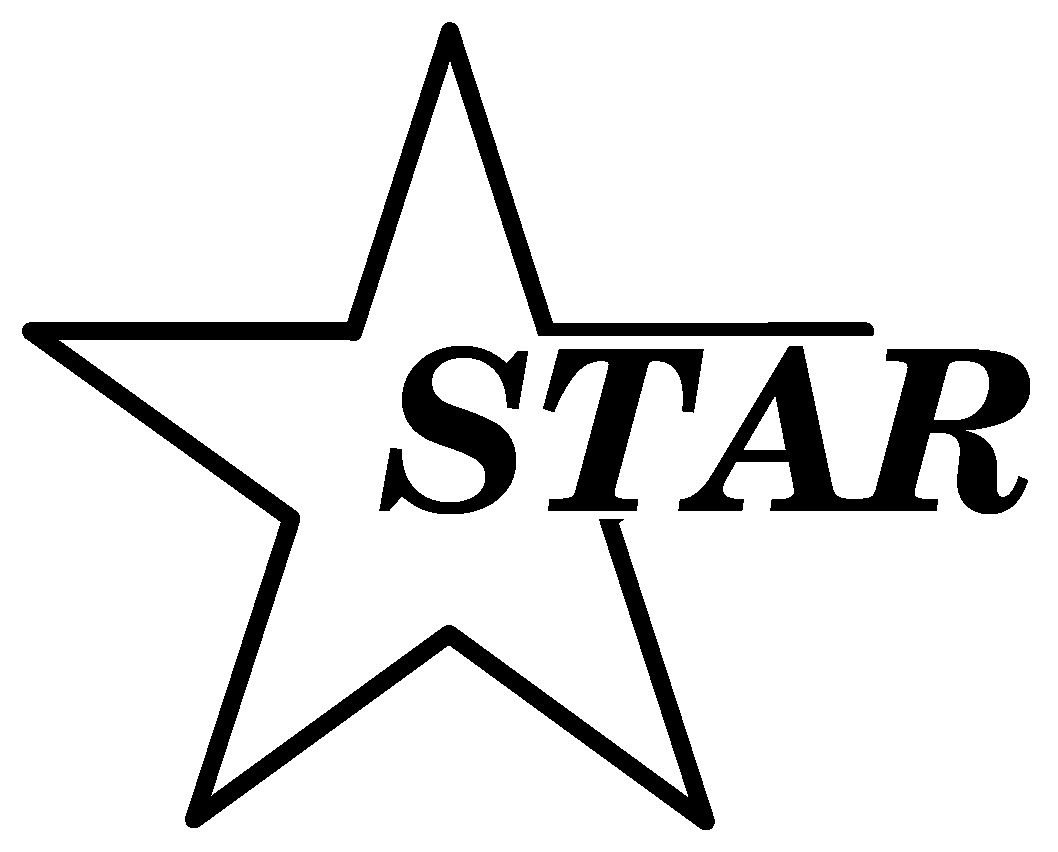
\includegraphics[width=2cm]{StarIcon.eps}}
  {\Large\bf STAR Offline Library Long Writeup}
  \hfill\mbox{}\\[3cm]
  \mbox{\includegraphics[width=\textwidth]{StMcEventTitle.eps}}
  \hfill\mbox{}\\[3cm]
  {\LARGE User Guide and Reference Manual}\\[2cm]
  {\LARGE $  $}  \\[5mm] % replaced by cvs with current revision
  {\LARGE $  $}  % replaced by cvs with current revision
  \vfill
\end{center}
\cleardoublepage
\end{titlepage}
\pagenumbering{roman}

%%%%%%%%%%%%%%%%%%%%%%%%%%%%%%%%%%%%%%%%%%%%%%%%%%%%%%%%%%%%%%%%%%%%
%
%    Table of contents
%
%%%%%%%%%%%%%%%%%%%%%%%%%%%%%%%%%%%%%%%%%%%%%%%%%%%%%%%%%%%%%%%%%%%%
\tableofcontents
\cleardoublepage

%%%%%%%%%%%%%%%%%%%%%%%%%%%%%%%%%%%%%%%%%%%%%%%%%%%%%%%%%%%%%%%%%%%%
%
%    User Guide
%
%%%%%%%%%%%%%%%%%%%%%%%%%%%%%%%%%%%%%%%%%%%%%%%%%%%%%%%%%%%%%%%%%%%%
\pagenumbering{arabic}
\part{User Guide}
\clearpage

%%%%%%%%%%%%%%%%%%%%%%%%%%%%%%%%%%%%%%%%%%%%%%%%%%%%%%%%%%%%%%%%%%%%

\section{Introduction}

\StMcEvent\footnote{We will adopt the convention used in \StEvent\ 
    and write \StMcEvent\ when we refer to the package and
    \name{StMcEvent} when we refer to the class.} is a package that
compliments the use of \StEvent\ . The aim is for the user to be able
to access and analyze Monte Carlo with the same object oriented
approach as \StEvent\ . The top class is \name{StMcEvent}, and a
pointer to this  class enables access to all the relevant Monte Carlo
information.  Again, the pointer is obtained through a Maker, in this
case \name{StMcEventMaker}.  An example invocation is found in sec.~\ref{sec:howto}.

The information contained in \StMcEvent\ is designed to be simply
a reflection of the information already available in the existing
g2t tables.  The primary keys and foreign keys are replaced by
associations between classes through pointers, like in \StEvent\ .
At the moment, not all the information found on the g2t tables is
encapsulated in \StMcEvent\ , for a full description of what is
avaliable, please refer to sec.~\ref{sec:refman}.  Also note that
\StMcEvent\ is a work in progress, and if additional information
is needed, it can be added.

The goal of \StMcEvent\ is to be used in conjunction with \StEvent\ in
order to have an OO model for both pure Monte Carlo data and DST data
that has passed through the whole reconstruction chain.  To be able
to relate the 2 packages, there is an additional package that is
run after both \StEvent\ and \StMcEvent\ are filled: \StAssociationMaker\ .
\index{StAssociationMaker}
The aim of \StAssociationMaker\ is to establish the relationships
between the reconstructed and Monte Carlo information, so that
users can easily check whether a particular reconstructed hit or
track is found, and if that is the case,
to directly obtain the associated Monte
Carlo hit or track so that an assessment of the quality of the
data can be made.

\clearpage

%%%%%%%%%%%%%%%%%%%%%%%%%%%%%%%%%%%%%%%%%%%%%%%%%%%%%%%%%%%%%%%%%%%%

\section{How to read this document}

This document is divided in two parts, a user guide and a
reference manual. In the first part we rather concentrate on basic
questions and provide guidance to get started.  Some of the information
given here overlaps that one found in the \StEvent\ documentation,
and we provide it again here for completeness (We think that it is better
to be redundant than to have to remember which information is in which
manual).  The reference section
provides information on all available classes, their member functions
and related operators. The class references contain one or more
examples which demonstrate some features of each class and how to use
them.

New users should \textbf{not} start with the Reference section. It is
meant as a lookup when specific information is needed. Beginners
should study the User Guide and should make themselves familiar only
with those classes they will encounter more frequently:
\name{StMcEvent}  (sec.~\ref{sec:StMcEvent}),
\name{StMcTrack}  (sec.~\ref{sec:StMcTrack}),
\name{StMcVertex} (sec.~\ref{sec:StMcVertex}),
\name{StMcTpcHit} (sec.~\ref{sec:StMcTpcHit}).
\name{StMcSvtHit} (sec.~\ref{sec:StMcSvtHit}).
and \name{StMcFtpcHit} (sec.~\ref{sec:StMcFtpcHit}).



Understanding the various
examples certainly is the best way to get started. However, the examples
are given for illustration purposes only, and are not complete programs.

%%%%%%%%%%%%%%%%%%%%%%%%%%%%%%%%%%%%%%%%%%%%%%%%%%%%%%%%%%%%%%%%%%%%

\section{Further documentation}
\label{sec:furtherdoc}

\StMcEvent\ makes use of various classes from the StarClassLibrary (SCL).
To obtain the SCL documentation, the easiest thing to do is to go to
the web page set up by Gene van Buren. 
Go to
\begin{verbatim}
http://www.star.bnl.gov/STARAFS/comp/root/special_docs.html
\end{verbatim}
Here you can easily obtain the documentation several packages
(this one for example).
\index{Gene's Documentation Page}
\index{SCL} \index{StarClassLibrary}

%%%%%%%%%%%%%%%%%%%%%%%%%%%%%%%%%%%%%%%%%%%%%%%%%%%%%%%%%%%%%%%%%%%%

\section{Getting \StMcEvent\ Sources}  \index{Getting StMcEvent sources}

To access the complete source code proceed as follows:

\StMcEvent\ is under {\bf CVS} control at BNL.  It can
be accessed via \name{afs}: \index{afs} \index{CVS} \index{CVSROOT}
\begin{enumerate}
  \item Obtain an \name{afs} token: \name{klog -cell rhic}.
  \item Make sure \name{\$CVSROOT} is set properly:\\ %%$
    (i.e.~\name{CVSROOT = /afs/rhic/star/packages/repository})
  \item Check-out package into your current working directory:\\
    \name{cvs checkout StRoot/StMcEvent}
\end{enumerate}

%%%%%%%%%%%%%%%%%%%%%%%%%%%%%%%%%%%%%%%%%%%%%%%%%%%%%%%%%%%%%%%%%%%%

\section{Coding Standards}
\index{Coding Standards}

\StMcEvent\ tries to follow the STAR coding guidelines as described on the
STAR $\rightarrow$ Computing $\rightarrow$ Tutorials $\rightarrow$ C++
coding standards web page: \\
http://www.star.bnl.gov/STAR/html/comp\_l/train/standards.html.\\
Here we
summarize the most relevant ones concerning the programmable interface:
\begin{itemize}
\item all classes, enumerations and functions start with the prefix
    \textbf{St}
\item all member functions start with a lowercase letter
\item header files have the extension \textbf{.hh}, source files have
    the extension\textbf{ .cc}
\item the use of underscores in names is discouraged
\item classes, methods, and variables have self-explanatory English
    names and first letter capitalization to delineate words
\end{itemize}

\StMcEvent\ also follows the following rules set forth in \StEvent\ 
\begin{itemize}
\item methods (member functions) which return a certain object have
    the same name as the referring object, i.e., without a preceding
    \name{get} prefix \\ (as in \name{StMcEvent::primaryVertex()})
\item methods which assign a value to a data member (or members) carry
    the prefix \name{set} followed by the name of the member (as in \name{StMcEvent::set\-Primary\-Vertex()}).
\item integer variables which serve as counter or indices and never
    can take negative values are consistently declared as
    \name{unsigned}.
\item Objects which are returned by pointer are not guaranteed to
    exist in which case a NULL pointer is returned. It is the user's
    responsibility to check for the return value and make sure the
    pointer is valid (non-zero) before she/he dereferences it.  Objects
    which are guaranteed to exist are returned by reference or by value.
\end{itemize}
%%%%%%%%%%%%%%%%%%%%%%%%%%%%%%%%%%%%%%%%%%%%%%%%%%%%%%%%%%%%%%%%%%%%
\section{Conventions}
\subsection{Numbering Scheme}
\label{sec:numberscheme}
\index{Numbering}
The information here is a reiteration of that found in the \StEvent\
Manual.  Both packages use the same conventions, but in order to
stress the difference between the official STAR numbering scheme
for subdetector components, and
the C/C++ conventions for indexing the containers with which we represent those
subdetectors, we repeat the cautions here.  The C/C++ convention
is that the first element in an array has the index 0.  This applies
to vectors, collections or other containers that allow indexing.
The TPC sectors and padrows,
the SVT layers, ladders and wafers, and the FTPC planes and sectors
all start counting at 1.  So it is important to remember this when
using the member functions that return the sector or padrow of a
TPC hit, for example, to address the elements in a container.  If
you want to obtain the hit container in which a particular hit
\verb+h+ is stored, you would do the following:

\begin{verbatim}
evt->tpcHitCollection()->sector(h.sector()-1)->padrow(h.padrow()-1).hits();
\end{verbatim}
Note the subtraction of 1, in order to index the array properly.
The functions that have this convention are:

\begin{itemize}
	\item \texttt{StMcTpcHit::sector()}
	\item \texttt{StMcTpcHit::padrow()}
	\item \texttt{StMcFtpcHit::plane()}
	\item \texttt{StMcSvtHit::layer()}
	\item \texttt{StMcSvtHit::ladder()}
	\item \texttt{StMcSvtHit::wafer()}
	\item \texttt{StMcSvtHit::barrel()}
	\item \texttt{StMcRichHit::pad()}
	\item \texttt{StMcRichHit::row()}
\end{itemize}

Note that in \StMcEvent\ there are no sectors for the FTPC.  This is due to the
fact that the determination of the sector for FTPC hits is strongly dependent
on the field and is done during reconstruction.  Therefore, FTPC hits
at the Monte Carlo level only know which plane they belong to, but know
nothing about sectors.

\subsection {References and Pointers}
Part of the goal of \StMcEvent\ is the use of pointers and references
as opposed to id's and foreign keys.  However, the handling of
pointers must be done with care.
To reiterate wise words of caution: If a function returns an object by
\textit{reference},
the object is guaranteed to exist.  If a function returns an object by {\it pointer},
then it is a good idea to always check if the pointer is \verb+NULL+. Not doing
this can be the cause of many a headache and sleepless nights.  This is one of
the most common ``monsters under the bed'' that can painfully bite, 
and crash code all over the place.

\subsection{Units}
\index{units} \index{system of units}
\label{sec:units}

All quantities in \StMcEvent\ are stored using the official STAR units:
cm, GeV and Tesla.  In order to maintain a coherent system of units it
is recommended to use the definitions in \name{SystemOfUnits.h} from
the StarClassLibrary. They allow to 'assign' a unit to a given
variable by multiplying it with a constant named accordingly
(centimeter, millimeter, kilometer, tesla, MeV, ...).  The value of
the constants is thus that the result after the multiplication follows
always the STAR system of units.

The following example illustrates their use:
{\footnotesize
\begin{verbatim}
double a = 10*centimeter;
double b = 4*millimeter;
double c = 1*inch;
double E1 = 130*MeV;
double E2 = .1234*GeV;

//
//   Print in STAR units
//
cout << "STAR units:" << endl;
cout << "a = " << a << " cm" << endl;
cout << "b = " << b << " cm" << endl;
cout << "c = " << c << " cm" << endl;
cout << "E1 = " << E1 << " GeV" << endl;
cout << "E2 = " << E2 << " GeV" << endl;

//
//   Print in personal units
//
cout << "\nMy units:" << endl;
cout << "a = " << a/millimeter << " mm" << endl;
cout << "b = " << b/micrometer << " um" << endl;
cout << "c = " << c/meter << " m" << endl;
cout << "E1 = " << E1/TeV << " TeV" << endl;
cout << "E2 = " << E2/keV << " keV" << endl;
\end{verbatim}
}%footnotesize
The resulting printout is:
{\footnotesize
\begin{verbatim}
STAR units:
a = 10 cm
b = 0.4 cm
c = 2.54 cm
E1 = 0.13 GeV
E2 = 0.1234 GeV

My units:
a = 100 mm
b = 4000 um
c = 0.0254 m
E1 = 0.00013 TeV
E2 = 123400 keV
\end{verbatim}
}%footnotesize

Further documentation can be found in the StarClassLibrary manual
(see sec.~\ref{sec:furtherdoc}).

\subsection{Containers and Iterators}
\label{sec:containers}
\index{containers}
\index{iterators}

The containers used throughout \StMcEvent\
\begin{itemize}
  \item are STL vectors (see below)\ref{subsec:vectors}.
  \item store objects by pointer.
\end{itemize}
Because the are {\tt vector}s, they allow random access as in:

\verb+pointer_to_object = container[index];+

The containers are guaranteed to provide the following member functions:
\name{size()}, \name{begin()}, \name{end()}.  All collections in
\StMcEvent\ have a referring iterator defined.
The containers and iterators are all declared in the file
{\tt StMcContainers.hh}, for convenience.  In addition,
all the classes in \StMcEvent\ are {\tt \#include}d in
the header {\tt StMcEventTypes.hh}.
\index{{\tt \#include} files}
\index{include files}
\index{StMcEventTypes}
The names given to the containers are meant to reflect
the objects contained, as well as whether a container is
a {\it structural} container or not.
\index{structural containers}
By a structural container we mean a container that owns the objects
it contains.  This means that when a structural container is deleted,
the objects it holds get deleted as well.  The naming convention
is then:

\begin{itemize}
  \item A {\bf vec}tor of {\bf p}oin{\bf t}e{\bf r}s
will carry the prefix {\bf \tt StPtrVec}
  \item A {\bf s}tructural {\bf vec}tor of {\bf p}oin{\bf t}e{\bf r}s
will carry the prefix {\bf \tt StSPtrVec}
\end{itemize}

The name is completed with the type of the objects they contain.  So
the structural container of pointers to objects of type \name{StMcTpcHit} is
\name{StSPtrVecMcTpcHit} where we drop the \name{St} of the object being
contained.

In reality, whether a container is structural or not
is of little importance in terms of its usage, the interface and methods of
both are the same.  The distinction is made to keep the objects organized,
and to make sure everthing gets deleted, and deleted in only one place.  But
this mainly goes on behind the scenes.  The main point one should
keep in mind from all of this is that, unless you really know
what you are doing, you should {\bf NOT} delete a
structural container.  (Play music for ``The Twilight Zone''.)


In order to keep your code independent of the underlying container
types, people are encouraged to use \textit{iterators} instead of
indices. These permit a higher degree of flexibility,
allowing to change containers
without changing the application code using them. The following
example demonstrates this:

Given an arbitrary \StMcEvent\ collection \name{anyColl} of type
\name{StAnyColl}
which holds objects of type \name{obj} the following code is
not guaranteed to work:
\begin{verbatim}
     for (int i=0; i<anyColl.size(); i++)
         obj = anyColl[i];
\end{verbatim}
A {\tt list} for example, does not allow random access, so indexing
is not supported for {\tt lists}.  For vectors and deques, indexing does work.
Iterators however, work for all STL containers.  The code above then,
should be replaced by:
\begin{verbatim}
     StAnyCollIterator iter;
     for (iter = anyColl.begin(); iter != anyColl.end(); iter++)
         obj = *iter;
\end{verbatim}

The names of the iterators defined in \StMcEvent\ are just the name
of the object contained + the word {\tt Iterator}.  For example,
the iterator for the container \name{StPtrVecMcVertex} is
\name{StMcVertexIterator}.

Note that all collections are by pointer, so they are
\textit{polymorphic} containers; that is, they are not restricted to
collect objects of the base type only, but can store
objects of any type derived from
the base. This is especially important when dereferencing the iterator to
access the objects in the collection.  Polymorphism is not
really used in \StMcEvent, but it is necessary in \StEvent, where,
for example, one has containers of tracks, but they can be Global
or Primary.  If a method returns a base class and one really wants
a derived class, we have to use Run Time Type Information (RTTI),
{\tt dynamic\_cast}ing and such.  Also, make sure you know how to
get the objects you want, depending on the type of objects in the
container.

For a \textit{by-pointer} collection:
\begin{verbatim}
     StMcVertexIterator iter;
     StSPtrVecMcVertex& vertices = event->vertices();
     StMcVertex* vertex;
     for (iter = vertices.begin(); iter != vertices.end(); iter++)
         vertex = *iter;                         // dereference once
\end{verbatim}

Hint: Use pointers or references to collection elements wherever
possible.  Making local copies is often time- and memory-intensive.
For example the same code above but written as:
\begin{verbatim}
     StMcVertexIterator iter;
     StMcVertexCollection* vertices = event->vertexCollection();
     StMcVertex vertex;
     for (iter = vertices->begin(); iter != vertices->end(); iter++)
         vertex = **iter;                         // dereference twice
\end{verbatim}
invokes the \name{StMcVertex} assignment operator and creates a local copy.
This method is only useful if you intend to modify an object locally
but want to leave the original untouched.

\subsubsection{Quick glance at {\tt vector}s}
\label{subsec:vectors}
As mentioned before, all containers used in \StMcEvent\ are STL {\tt vectors}.  That
means that one can use the methods supported by the {\tt vector}
template class.  I'll give a brief overview of some basic elements
of {\tt vector}s to provide some common ground on which to walk on, for
people unfamiliar with the STL.  A LOT more information can be found
in your favorite C++ book.
\index{vector}

\paragraph{Common Member Types}
The type of the elements of the container is passed as the
first template argument, and is known as its {\tt value\_type}.  For
example, the {\tt value\_type} of the \name{StPtrVecMcTrack} container,
which is really a \verb+vector<StMcTrack*>+ is, of course, {\tt StMcTrack*}.
The type used for indexing into the container is known as {\tt size\_type},
and {\tt difference\_type} is the type of the result of subtracting
two iterators.  Like mentioned before, every container defines an
{\tt iterator} and a {\tt const\_iterator} for pointing to the elements
of the container.  One of the aims of these types is to allow the
possibility to write code without knowing the actual types involved.

\paragraph{Public Member Functions}
The following methods illustrate some of the methods provided by
the {\tt vector} container.  The list is by no means complete, but
even so there are some more methods listed here than normally used.
The counterpart {\tt const} methods are omitted.
\begin{Entry}
\item[Iterator Methods]
  \verb+iterator  begin()+\\
  Points to the first element of the container.

  \verb+iterator  end()+\\
  Points to the last-plus-one element.

  \verb+reverse_iterator  rbegin()+\\
  Points to the first element of the reverse sequence.
  Note that the
  type of the iterator is different than for {\tt begin()}.
  Useful when going through a sequence backwards.  For more
  information on {\tt reverse\_iterator} consult your favorite
  C++ reference book.
  
  \verb+reverse_iterator  rend()+\\
  Points to the last-plus-one element of the reverse sequence.

\end{Entry}

The following methods allow to access the elements of the container.

\begin{Entry}

\item[Useful Access \\Methods]

  \verb+reference  operator[](size_type n)+\\
  Provides unchecked access to the elements of the container.  Safe
  to use when there is a previous condition to guarantee that
  the argument is within bounds.

  \verb+reference  at(size_type n)+\\
  Provides range checked access to the elements of the container.\\
  Throws {\tt out\_of\_range} if the index is out of range.

  \verb+reference  front()+\\
   Reference to the first element of the container.
  
  \verb+reference  back()+\\
   Reference to the last element of the container.

  \verb+size_type  size()+\\
   Number of elements in the container.  

  \verb+void  push_back(const T& x)+\\
  Adds the element to the end of the container, {\tt size()} increases
  by 1.

  \verb+void  pop_back(const T& x)+\\
  Removes the last element of the container, {\tt size()} decreases
  by 1.

  \verb+void  clear()+\\
  Erases all the elements.

\end{Entry}


%%%%%%%%%%%%%%%%%%%%%%%%%%%%%%%%%%%%%%%%%%%%%%%%%%%%%%%%%%%%%%%%%%%%

\section{How to use \StMcEvent: The Macro and the Maker}
\label{sec:howto}
\subsection{StMcEventReadMacro.C}
\index{StMcEventReadMacro.C}
\index{root4star}
\index{ROOT files}
\StMcEvent\ has now been a package in the STAR library for a while.  The
new version which this guide refers to is, as of this writing,
available in starnew and stardev.  Remember, that libraries
get moved, so make sure you are using the right library for
your purposes.  This is very important, since to use \StMcEvent\
along with \StEvent\ one CANNOT combine the latest code with
files produced before December 1999, since the dst tables
and \StEvent\ changed substantially.

To run the example macro StMcEventReadMacro.C, one can just
run the default version directly from the library:
\begin{verbatim}
    stardev
    cd somewhere
    root4star -b
    .x StMcEventReadMacro.C
\end{verbatim}
This will run the macro in the repository with the default settings:
Process one event from the default geant.root file, load StMcEvent
and print out to the screen some information on the event.
If this step doesn't work, then something weird is going on.  (Although
make sure if you are using dev that Lidia is not rebuilding the whole
library while you are trying to run one of the examples!)  The
default macros are meant to work ``out of the box'', so to speak,
so this is the first step to check that things are working
properly.

The next step is to actually check out the macro and edit it yourself for
your purposes.  To check out the macro, do the following:
\begin{verbatim}
    klog
    mkdir workdir
    cd workdir
    cvs co StRoot/macros/examples/StMcEventReadMacro.C
\end{verbatim}

StMcEventReadMacro.C is found in
\name{\$CVSROOT/StRoot/macros/examples/StMcEventReadMacro.C},  %$
and it runs a chain runs a chain of just one maker to load \StMcEvent .


%%%%%%%%%%%%%%%%%%%

At the moment, it runs the chain on a ROOT file tree.  That is, it uses
the GEANT branches of the files it finds in the directory.  This is important to
realize if you want to run the macro on files other than the default, an
activity one should quickly graduate to.  The macro takes as arguments the
number of events to process, and the name of the file to be used.  An example invocation
is:

{\footnotesize

\begin{verbatim}

.x StMcEventReadMacro.C(10,"/star/rcf/test/dev/tfs_Linux/Mon/year_2a/hc_standard/*.geant.root")
     

\end{verbatim}
}
This invocation will process 10 events from the specified file.
Now, to open the files, branches, etc. we rely on StIOMaker.  This maker
takes the path to look for files from the specified file, but the files
it actually
opens depend on
what branches are activated in the macro.
This is done inside the macro with the command \name{SetBranch}.

\subsection{StMcEventMaker}
\index{StMcEventMaker}
\name{StMcEventMaker} is the code that actually does the opening of
the geant.root file and uses the information there to set up the
whole \StMcEvent .  If you want to use \StMcEvent\ you have to make
sure that \name{StMcEventMaker} is instantiated in the chain you
are running.  This will take care of all the setup.  The data
members and methods of the maker that you will be useful are:

\index{StMcEventMaker|textbf}
\label{sec:StMcEventMaker}
\begin{Entry}
\item[Synopsis]
    \verb+#include "StMcEventMaker.hh"+\\
    \verb+class StMcEventMaker;+\\

\item[Public Data\\ Members]
    \verb+Bool_t  doPrintEventInfo;+\\
    Print or do not print info on the current \StMcEvent\ event.
    (default=kFALSE).  This produces a lot of output, and is
    meant for debugging.  Every major
    class is dumped, the sizes of all collections, and the first
    element in every container. Don't use it for production.
    
    \verb+Bool_t  doPrintMemoryInfo;+\\
    Switch on/off checks on memory usage of \StMcEvent\
    (default=kFALSE).  In order to get a memory snapshot we use
    \texttt{StMemoryInfo} from the \name{StarClassLibrary}.  A
    snapshot is taken before and after the setup of \StEvent.  The
    numbers in brackets refer to the difference. Not available on SUN
    Solaris yet.
    
    \verb+Bool_t  doPrintCpuInfo;+\\
    Switch on/off CPU usage (default=kFALSE). Tells you how long it
    took to setup \StEvent. Timing is performed using \texttt{StTimer}
    from the StarClassLibrary.

\item[Public Member\\ Functions]
    \verb+StMcEvent*  currentMcEvent();+\\
    Returns a pointer to the current \name{StMcEvent} object.
\end{Entry}

Since the \name{StMcEvent} object you get when you invoke
{\tt currentMcEvent()} is held by pointer, dont forget to
check if this is {\tt NULL}. This would immediately signal
something gone awry.  Also, do not delete the objects
you get from the StMcEvent methods, they will be deleted
every time you read a new event.

In order to use the classes in
\StMcEvent\ in other Makers, one header file with {\it all} the include files
is provided: {\tt StMcEventTypes.hh}. \index{StMcEventTypes}
Like with \StEvent\ this makes
life easier in terms of not having to remember which file you need where,
you just care about one include file and that's it.  
\index{{\tt \#include} files}
\index{include files}
The next step is the use of the \StAssociationMaker\ package.  This is described
in its own manual.

%%%%%%%%%%%%%%%%%%%%%%%%%%%%%%%%%%%%%%%%%%%%%%%%%%%%%%%%%%%%%%%%%%%%

\section{Known Problems and Fixes}
\index{known problems and fixes}

\StMcEvent\ is changing as the software environment changes.  From the last
version, several things have been updated and the design revamped to
follow \StEvent\ .
The creation of the vertex collection from the tables took its final
form, once the g2t\_vertex table was corrected.  The g2t\_event table was
finally written out, so it is now available.

The FTPC and SVT associations between reconstructed and Monte Carlo
hits are now included.
Also, the problems \StAssociationMaker\ had with the declaration of multimaps
by the Solaris CC4.2 compiler (i.e. no Template Default Arguments, and
ObjectSpace implementation of the STL) have been solved and
now \StMcEvent\ and \StAssociationMaker\ compile and run
on Linux gcc, Solaris CC4.2 and CC5 and HP aCC.

For corrections to this manual, typos, suggestions, etc. send an email
to {\tt calderon@star.physics.yale.edu}.
\clearpage

%%%%%%%%%%%%%%%%%%%%%%%%%%%%%%%%%%%%%%%%%%%%%%%%%%%%%%%%%%%%%%%%%%%%
%
%    Reference Manual
%
%%%%%%%%%%%%%%%%%%%%%%%%%%%%%%%%%%%%%%%%%%%%%%%%%%%%%%%%%%%%%%%%%%%%
\part{Reference Manual}
\label{sec:refman}
\clearpage

%%%%%%%%%%%%%%%%%%%%%%%%%%%%%%%%%%%%%%%%%%%%%%%%%%%%%%%%%%%%%%%%%%%%

\section{Global Constants}

We use the constants defined in the two header files
\index{StarClassLibrary} \name{SystemOfUnits.h} and
\name{PhysicalConstants.h} which are part of the StarClassLibrary.
The types defined therein are used
throughout \StMcEvent\ .



%%%%%%%%%%%%%%%%%%%%%%%%%%%%%%%%%%%%%%%%%%%%%%%%%%%%%%%%%%%%%%%%%%%%

\section{Class Reference}
The classes which are currently implemented and available from the
STAR CVS repository are described in alphabetical order.

Inherited member functions and operators are not described in the
reference section of a derived class. Always check the section(s)
of the base class(es) to get a complete overview on the available
methods.

Note that some constructors are omitted, especially the ones which
take tables as arguments. They are for internal use only (even if
public).

Destructors, assignment operators and copy constructors are not
listed.  Macros and \name{Inline} declarations are omitted throughout the
documentation, as well as the {\tt virtual} keyword.  For the
most up-to-date reference of what is available, there is no
substitute to looking directly at the class definition in
the header file.

\clearpage


%%%%%%%%%%%%%%%%%%%%%%%%%%%%%%%%%%%%%%%%%%%%%%%%%%%%%%%%%%%%%%%%%%%%
%
%    Reference: StMcEvent
%
%%%%%%%%%%%%%%%%%%%%%%%%%%%%%%%%%%%%%%%%%%%%%%%%%%%%%%%%%%%%%%%%%%%%
\subsection{StMcEvent}
\index{StMcEvent|textbf}
\index{event header}
\label{sec:StMcEvent}
\begin{Entry}
\item[Summary]
    \name{StMcEvent} is the top class in the \StMcEvent\ data model.
    It provides methods to access all quantities and objects
    stored in the g2t tables.

\item[Synopsis]
    \verb+#include "StMcEvent.hh"+\\
    \verb+class StMcEvent;+\\

\item[Description]
    Objects of type \name{StMcEvent} are the entry point to the g2t data.
    From here one can navigate to (and access) quantities stored
    in the g2t tables, but instead of going through foreign keys and
     Id's all relationships are established through pointers. 
    The only {\tt \#include} file needed to access all the classes of \StMcEvent\
    is the {\tt StMcEventTypes.hh} file. \index{StMcEventTypes}
    \name{StMcEvent} itself doesn't offer much functionality but rather serves
    as a container for the event data.
    Deleting \name{StMcEvent} deletes the whole data tree, i.e.~all depending objects
    are deleted properly.

\item[Persistence]
    None

\item[Related Classes]
    None

\item[Public\\ Constructors]
    \verb+StMcEvent();+\\
    Default constructor. Creates an "empty" event.  Normally not used.  As with
    most other classes, the constructor used normally is based on g2t tables.

\item[Public Member\\ Functions]
    

    \verb+unsigned long eventGeneratorEventLabel() const;+\\
    Event Label from event generator, read from g2t\_event.
    \index{event generator label}

    \verb+unsigned long eventNumber() const;+\\
    Event number from monte carlo production, read from g2t\_event.
    \index{event number}

    \verb+unsigned long runNumber() const;+\\
    Run number, read from g2t\_event.
    \index{run number}

    \verb+unsigned long zWest() const;+\\
    Number of protons of particle coming from the ``West'', read from g2t\_event.
    \index{zWest}

    \verb+unsigned long nWest() const;+\\
    Number of neutrons of particle coming from the ``West'', read from g2t\_event.
    \index{nWest}

    \verb+unsigned long zEast() const;+\\
    Number of protons of particle coming from the ``East'', read from g2t\_event.
    \index{zEast}

    \verb+unsigned long nEast() const;+\\
    Number of neutrons of particle coming from the ``East'', read from g2t\_event.
    \index{nEast}

    \verb+unsigned long numberOfPrimaryTracks() const;+\\
    Number of primary tracks read from g2t\_event.  Note that this is
    not coming from {\tt primaryVertex()->daughters().size()} so one
    can check whether these numbers are actually the same.
    \index{primary tracks}

    \verb+float impactParameter() const;+\\
    Impact parameter of collision, read from g2t\_event.
    \index{impact parameter}

    \verb+float phiReactionPlane() const;+\\
    Phi angle of the reaction plane of the collision, read from g2t\_event.
    \index{phi reaction plane}

    \verb+float triggerTimeOffset() const;+\\
    Trigger time offset, read from g2t\_event.
    \index{trigger time offset}

    \verb+StMcVertex* primaryVertex();+\\
    Returns a pointer to primary vertex. The same object is stored
    in the \name{StMcVertexCollection}. Since the primary vertex is of
    high importance for most analysis steps, this method was added
    for convenience. Note that if no primary vertex is available
    this function returns a {\tt NULL} pointer, so be careful!
    \index{primary vertex}

    \verb+StSPtrVecMcVertex& vertices();+\\
    Returns a reference to the vertex container, i.e., the {\tt vector} of all
    event vertices.
    \index{vertex container}  
    \verb+StSPtrVecMcTrack& tracks();+\\
    Returns reference to the track container, i.e., the {\tt vector} of all
    monte carlo tracks.
    \index{track container}

    \verb+StMcTpcHitCollection* tpcHitCollection();+\\ 
    Returns a pointer to the TPC hit collection.  Note that the
    collections are {\emph NOT} just flat containers.  The TPC hit
    collection is a container of sectors.  The sectors are containers
    of padrows, where the TPC hits are stored.
    \index{hit collections, TPC}

    \verb+StMcSvtHitCollection* svtHitCollection();+\\
    Returns a pointer to the SVT hit collection.  The SVT hit
    collection is a container of layers.  The layers are containers
    of ladders.  The ladders are containers of wafers,
    where the SVT hits are stored.
    \index{hit collections, SVT}


    \verb+StMcFtpcHitCollection* ftpcHitCollection();+\\
    Returns a pointer to the FTPC hit collection. The FTPC hit
    collection is a container of planes.  Note that it is in the planes 
    where the FTPC hits are stored.  The Monte Carlo hits of the FTPC
    know nothing about sectors, because these are only determined
    after reconstruction.
    \index{hit collections, FTPC}


    The following member functions are used to set data members of \name{StMcEvent}.
    They are shown only for completeness and shouldn't be used without
    a profound understanding of the relations between the different objects.

    \verb+void setEventGeneratorEventLabel(unsigned long);+\\
    \verb+void setEventNumber(unsigned long);+\\
    \verb+void setRunNumber(unsigned long);+\\
    \verb+void setZWest(unsigned long);+\\
    \verb+void setNWest(unsigned long);+\\
    \verb+void setZEast(unsigned long);+\\
    \verb+void setNEast(unsigned long);+\\
    \verb+void setImpactParameter(float);+\\
    \verb+void setPhiReactionPlane(float);+\\
    \verb+void setTriggerTimeOffset(float);+\\
    \verb+void setPrimaryVertex(StMcVertex*);+\\
    \verb+void setTrackCollection(StMcTrackCollection*);+\\
    \verb+void setTpcHitCollection(StMcTpcHitCollection*);+\\
    \verb+void setSvtHitCollection(StMcSvtHitCollection*);+\\
    \verb+void setFtpcHitCollection(StMcFtpcHitCollection*);+\\
    \verb+void setVertexCollection(StMcVertexCollection*);+\\

\item[Public Member\\ Operators]
    \verb+int operator==(const StMcEvent&) const;+\\
    Compares the event number, run number and type to determine
    whether 2 events are equal.

    \verb+int operator!=(const StMcEvent&) const;+\\
    Uses {\tt operator==} and negates it.

    \verb+ostream&  operator<<(ostream& os, const StMcEvent&);+\\
    Allows to write some relevant information directly to an output
    stream.

\item[Examples]
{\bf Example:}
{\footnotesize
\begin{verbatim}
//
//   Prints some basic event quantities to stdout (cout).
//   
//
void printEvent(StMcEvent *event)
{
     
     cout << "Event Generator Label = "
          <<  event->eventGeneratorEventLabel() << endl;
     cout << "Event Number = "
          <<  event->eventNumber() << endl;
     cout << "Run number = " << event->runNumber();
     cout << "# of tracks = "
          << event->trackCollection()->size() << endl;
     cout << "# of vertices = "
          << event->vertexCollection()->size() << endl;
     cout << "# of tpc hits = "
          << event->tpcHitCollection()->size() << endl;
     cout << "xyz of primary Vertex = "
          <<  event->primaryVertex()->position()/millimeter
          << " mm" << endl;
}

\end{verbatim}
}%footnotesize


\end{Entry}
\clearpage

%%%%%%%%%%%%%%%%%%%%%%%%%%%%%%%%%%%%%%%%%%%%%%%%%%%%%%%%%%%%%%%%%%%%
%
%    Reference: StMcFtpcHit
%
%%%%%%%%%%%%%%%%%%%%%%%%%%%%%%%%%%%%%%%%%%%%%%%%%%%%%%%%%%%%%%%%%%%%
\subsection{StMcFtpcHit}
\index{FTPC hit} \index{StMcFtpcHit|textbf}
\label{sec:StMcFtpcHit}
\begin{Entry}
\item[Summary]
    \name{StMcFtpcHit} represents a FTPC hit.

\item[Synopsis]
    \verb+#include "StMcFtpcHit.hh"+\\
    \verb+class StMcFtpcHit;+\\

\item[Description]
    \name{StMcFtpcHit} inherits most functionality from \name{StMcHit}.  For a complete
    description of the inherited member functions see \name{StMcHit}
    (sec.~\ref{sec:StMcHit}).

    In the \StMcEvent\ data model each track keeps references to the
    associated hits and vice versa. All hits have a pointer to their
    parent track.  This is especially important for the making of the
    associations in \StAssociationMaker.


\item[Persistence]
    None

\item[Related Classes]
    \name{StMcFtpcHit} is derived directly from \name{StMcHit}.
    The hits are kept according to sector.
    They are stored by pointer in a container for each sector
    (see \ref{sec:containers}).  The way to get the hits for a
    certain plane (1-20) starting
    from the top level \name{StMcEvent} pointer is:
    \verb+mcEvt->ftpcHitCollection()->plane(1)->hits()+
    Look in \ref{sec:StMcFtpcHitCollection} and
    \ref{sec:StMcFtpcPlaneHitCollection} for more information.
    Each instance of \name{StMcTrack} holds a list of FTPC hits
    which belong to that track.
    \index{StMcHit}
    \index{StMcTrack}
    \index{StMcFtpcHitCollection}

\item[Public\\ Constructors]
    \verb+StMcFtpcHit(const StThreeVector<float>& p,+\\
    \verb+          const float de, const float ds,+\\
    \verb+          StMcTrack* parent);+\\
    Create an instance of \name{StFtpcHit} with position \name{p},
    energy deposition at hit \name{de}, path length (within padrow) \name{ds},
    and parent track \name{parent}.  Not used.  Standard use is
    to obtain all parameters from g2t\_fpt\_hit table.

\item[Public Member\\ Functions]

    \verb+unsigned long plane() const;+\\
    Returns the number of the plane (1-20) in which a hit is found. 
    \index{plane, FTPC}

\item[Public Member\\ Operators]
    \verb+ostream&  operator<<(ostream& os, const StMcFtpcHit\&);+\\
    Allows to write some relevant information directly to an output
    stream.

\item[Examples]
{\footnotesize
\begin{verbatim}
//
//  In this example, we use the methods of the class
//  to access the data.  For concreteness, we use them to fill
//  a Root histogram. 
//  
void
PositionOfHits(StMcTrack *track)
{
   StPtrVecMcFtpcHit hits = track->ftpcHits();

   StMcFtpcHitIterator i;
   StMcFtpcHit* currentHit;
   TH2F* myHist = new TH2F("coords. MC","X vs Y pos. of Hits",100, -150, 150, 100, -150, 150)
   for (i = hits.begin(); i != hits.end(); i++) {
      currentHit = (*i);
      myHist->Fill(currentHit->position().x(), currentHit->position().y());
   }
}
\end{verbatim}
}%footnotesize
\end{Entry}

\clearpage
%%%%%%%%%%%%%%%%%%%%%%%%%%%%%%%%%%%%%%%%%%%%%%%%%%%%%%%%%%%%%%%%%%%%
%
%    Reference: StMcFtpcHitCollection
%
%%%%%%%%%%%%%%%%%%%%%%%%%%%%%%%%%%%%%%%%%%%%%%%%%%%%%%%%%%%%%%%%%%%%
\subsection{StMcFtpcHitCollection}
\index{FTPC hit collection} \index{StMcFtpcHitCollection|textbf}
\label{sec:StMcFtpcHitCollection}
\begin{Entry}
\item[Summary]
    \name{StMcFtpcHitCollection} is a container for the
    planes of the FTPC.  The actual hits are stored according to
    planes.

\item[Synopsis]
    \verb+#include "StMcFtpcHitCollection.hh"+\\
    \verb+class StMcFtpcHitCollection;+\\

\item[Description]
    \name{StMcFtpcHitCollection} is the first step down
    the hierarchy of hits for the FTPC.  It provides
    methods to return a particular plane, and to
    count the number of hits in all the FTPC.

\item[Persistence]
    None

\item[Related Classes]
    \name{StMcFtpcHitCollection}
    has a container of type {\tt StMcFtpcPlaneHitCollection}
    of size 20, each element represents a plane.
    \index{StMcFtpcPlaneHitCollection}
    \index{StMcFtpcHit}

\item[Public\\ Constructors]
    \verb+StMcFtpcHitHitCollection();+\\
    Create an instance of \name{StFtpcHitCollection}
    and sets up the internal containers.

\item[Public Member\\ Functions]

    \verb+bool addHit(StMcFtpcHit*);+\\
    Adds a hit to the collection (using \name{StMemoryPool}
    from the StarClassLibrary.

    \verb+unsigned long numberOfHits() const;+\\
    Counts the number of hits of the whole FTPC.

    \verb+unsigned int  numberOfPlanes() const;+\\
    Returns the size of the Array of planes.  Default is 20.

    \verb+StMcFtpcPlaneHitCollection*       plane(unsigned int);+\\
    Returns a pointer to the plane specified by the argument to the
    function.  Recall that this is for indexing into an array, so the
    argument should go from 0 - (size()-1).  Look in the
    numbering scheme conventions \ref{sec:numberscheme}for more information.

\item[Examples]
{\footnotesize
\begin{verbatim}
//
// Look in StMcFtpcPlaneHitCollection for an example.
// These classes normally go hand in hand.
\end{verbatim}
}%footnotesize
\end{Entry}

\clearpage
%%%%%%%%%%%%%%%%%%%%%%%%%%%%%%%%%%%%%%%%%%%%%%%%%%%%%%%%%%%%%%%%%%%%
%
%    Reference: StMcFtpcPlaneHitCollection
%
%%%%%%%%%%%%%%%%%%%%%%%%%%%%%%%%%%%%%%%%%%%%%%%%%%%%%%%%%%%%%%%%%%%%
\subsection{StMcFtpcPlaneHitCollection}
\index{FTPC plane hit collection} \index{StMcFtpcPlaneHitCollection|textbf}
\label{sec:StMcFtpcPlaneHitCollection}
\begin{Entry}
\item[Summary]
    \name{StMcFtpcPlaneHitCollection} is the class where the FTPC hits
    are actually stored.

\item[Synopsis]
    \verb+#include "StMcFtpcPlaneHitCollection.hh"+\\
    \verb+class StMcFtpcPlaneHitCollection;+\\

\item[Description]
    \name{StMcFtpcPlaneHitCollection} holds the FTPC hits.  Note
    the difference with \StEvent.  The Monte Carlo doesn't know
    about the sectors of the FTPC, these are determined during
    reconstruction.

\item[Persistence]
    None

\item[Related Classes]
    \name{StMcFtpcPlaneHitCollection}
    has a container of type {\tt StSPtrVecMcFtpcHit}, this means
    that this is the class that actually owns the hits.  Look
    at the section on containers \ref{sec:containers} for more
    information.    
    \index{StMcFtpcHit}
    \index{StSPtrVecMcFtpcHit}
\item[Public\\ Constructors]
    \verb+StMcFtpcPlaneHitCollection();+\\
    Create an instance of \name{StFtpcHitCollection}
    and sets up the internal container.

\item[Public Member\\ Functions]

    \verb+unsigned long numberOfHits() const;+\\
    Counts the number of hits of this plane.

    \verb+StSPtrVecMcFtpcHit&       hits();+\\
    Returns a reference to the container of the FTPC hits.
    
\item[Examples]
{\footnotesize
\begin{verbatim}
//
// Print number of hits in FTPC and plot 1D Histogram of r (cylindrical coord.) of
// Hits
//  
   StMcFtpcHitCollection* ftpcHitColl = evt->ftpcHits();
   cout << ``There are :`` << ftpcHitColl->numberOfHits() << ``hits in the FTPC'' << endl; 
   TH1F* myHist = new TH1F("Sector 10 ","R pos. of Hits",100, 0, 100)
   for (unsigned int i=0; i<ftpcHitColl->numberOfPlanes(); i++) {
     StSPtrVecMcFtpcHit& hits = ftpcHitColl->plane(i)->hits();
     for (StMcFtpcHitIterator i = hits.begin(); i != hits.end(); i++) {
       currentHit = (*i);
       myHist->Fill(currentHit->position().perp());
     }
   }
\end{verbatim}
}%footnotesize
\end{Entry}

\clearpage
%%%%%%%%%%%%%%%%%%%%%%%%%%%%%%%%%%%%%%%%%%%%%%%%%%%%%%%%%%%%%%%%%%%%
%
%    Reference: StMcHit
%
%%%%%%%%%%%%%%%%%%%%%%%%%%%%%%%%%%%%%%%%%%%%%%%%%%%%%%%%%%%%%%%%%%%%
\subsection{StMcHit}
\index{StMcHit|textbf} \index{hit}
\label{sec:StMcHit}
\begin{Entry}
\item[Summary]
    \name{StMcHit} is the base class of all TPC, FTPC, SVT and RICH
    monte carlo hit classes.

\item[Synopsis]
    \verb+#include "StMcHit.hh"+\\
    \verb+class StMcHit;+\\

\item[Description]
    \name{StMcHit} provides the basic functionality for all derived classes
    which represent TPC, FTPC SVT and RICH hits. It provides information on
    position, energy deposition, path length within sensitive volume,
    and the track which
    generated this hit.  All information is taken from
    the appropriate \name{g2t\_xxx\_hit.idl} table, where xxx can be ``tpc'', ``svt'',
    ``ftp'', or ``rch''.
    \name{StMcHit} is a virtual class.
    \index{g2t\_xxx\_hit.idl}

\item[Persistence]
    None

\item[Related Classes]
    The following classes are derived from \name{StMcHit}:
    \begin{itemize}
    \item \name{StMcTpcHit}
    \item \name{StMcFtpcHit}
    \item \name{StMcSvtHit}
    \item \name{StMcRichHit}
    \end{itemize}
    \index{StMcTpcHit}
    \index{StMcFtpcHit}
    \index{StMcSvtHit}
    \index{StMcRichHit}

\item[Public\\ Constructors]
    \verb+StMcHit();+\\
    Constructs an instance of \name{StMcHit} with all values initialized
    to 0 (zero).  Not used.  Normally, all hits belong to a certain detector,
    so the appropriate table based constructor is used.

    \verb+StMcHit(const StThreeVector<float>& p,+\\
    \verb+      float de, float ds, StMcTrack* parent);+\\
    
    Create an instance of \name{StMcHit} with position \name{p},
    energy deposition \name{de}, path length \name{ds}, and parent track \name{parent}.

\item[Public Member\\ Functions]
    \verb+const StThreeVectorF& position() const;+\\
    Hit position in global coordinates.

    \verb+float dE() const;+\\
    Energy deposition.

    \verb+float dS() const;+\\
    Path length within sensitive volume.

    \verb+StMcTrack* parentTrack() const;+\\
    Pointer to the track that generated the hit.

    The following functions should not normally be used.
    The relevant data members are set during construction or
    in \name{StMcEventMaker} so these are provided for completeness.

    \verb+void setPosition(const StThreeVectorF&);+\\
    Set the hit position.

    \verb+void setdE(float);+\\
    Set the total energy deposition.

    \verb+void setdS(float);+\\
    Set the path length within sensitive volume.

    \verb+void setParentTrack(StMcTrack*);+\\
    Set the parent track.
    
\item[Global Operators]

    \verb+int operator==(const StMcHit&) const;+\\
    Checks to see if 2 hits are equal.  Uses position, dE and dS
    for the comparison.

    \verb+int operator!=(const StMcHit&) const;+\\
    Uses operator== and negates the result.

    \verb+ostream&  operator<<(ostream& os, const StMcHit&);+\\
    Prints hit data (position, dE, dS ) to output stream \name{os}.

\item[Examples]
{\footnotesize
\begin{verbatim}
//
//  Create a random hit and print it.
//
void printArbitraryHit()
{
   HepJamesRandom engine;
   RandFlat       rndm(engine);
   RandGauss      rgauss(engine);
   const double   sigmadE = 1e-06;
   const double   sigmadS = 7*millimeter;
   StMcTrack* pTrack = new StMcTrack;

   StThreeVectorF pos(rndm.shoot(-meter,meter),
                            rndm.shoot(-meter,meter),
                            rndm.shoot(-meter,meter));
   float de = rgauss.shoot(2.0e-06,sigmadE);
   float ds = rgauss.shoot(1.6,sigmadS);
   StMcHit hit(pos, de, ds, pTrack);

   cout << hit << endl;
}
\end{verbatim}
}%footnotesize
{\bf Programs Output:}
{\footnotesize
\begin{verbatim}
Position: (-20.3111, -80.7543, 76.8227)
dE: 1.0952e-06
dS: 1.3049
\end{verbatim}
}%footnotesize

\end{Entry}
\clearpage
%%%%%%%%%%%%%%%%%%%%%%%%%%%%%%%%%%%%%%%%%%%%%%%%%%%%%%%%%%%%%%%%%%%%
%
%    Reference: StMcRichHit
%
%%%%%%%%%%%%%%%%%%%%%%%%%%%%%%%%%%%%%%%%%%%%%%%%%%%%%%%%%%%%%%%%%%%%
\subsection{StMcRichHit}
\index{RICH hit} \index{StMcRichHit|textbf}
\label{sec:StMcRichHit}
\begin{Entry}
\item[Summary]
    \name{StMcRichHit} represents a monte carlo RICH hit.

\item[Synopsis]
    \verb+#include "StMcRichHit.hh"+\\
    \verb+class StMcRichHit;+\\

\item[Description]    
    \name{StMcRichHit} inherits most functionality from \name{StMcHit}.
    For a complete description of the inherited member functions see
    \name{StMcHit} (sec.~\ref{sec:StMcHit}).

    In the \StMcEvent\ data model each track keeps references to the
    associated hits and vice versa. All hits have a pointer to their
    parent track.  This is especially important for the making of the
    associations in \StAssociationMaker. 
    
    
    
\item[Persistence]
    None

\item[Related Classes]
    \name{StMcRichHit} is derived directly from \name{StMcHit}.
    The hits are kept according to row and pad.
    The hits are kept in an instance of \name{StSPtrVecMcRichHit}
    where they are stored by pointer (see \ref{sec:containers}).
    Each instance of \name{StMcTrack} holds a list of RICH hits
    which belong to that track.
    \index{StMcHit}
    \index{StMcTrack}
    \index{StMcRichHitCollection}

\item[Public\\ Constructors]
    \verb+StMcRichHit(const StThreeVectorF& p,+\\
    \verb+      float de, float ds, StMcTrack* parent);+\\
    
    Create an instance of \name{StMcRichHit} with position \name{p},
    energy deposition \name{de}, path length \name{ds}, and parent track \name{parent}.

\item[Public Member\\ Functions]

    \verb+unsigned short  pad() const;+\\
    Returns the number of the pad in which a hit is found. 
    \index{pad, RICH}

    \verb+unsigned short  row() const;+\\
    Returns the number of the row in which a hit is found. 
    \index{row, RICH}

\item[Examples]
{\footnotesize
\begin{verbatim}
//
//  Function which returns the RICH hits
//  used by a track and prints them.
//
void getHits(StMcTrack *track)
{
    StPtrVecMcRichHit& hits =
                   track->richHits();
    StMcRichHitIterator iter;
    StMcRichHit* hit;
    for(iter = hits->begin();
        iter != hits->end(); iter++) {
        hit = *iter;
        cout << hit << endl;
    }
    
}
\end{verbatim}
}%footnotesize
\end{Entry}
\clearpage
%%%%%%%%%%%%%%%%%%%%%%%%%%%%%%%%%%%%%%%%%%%%%%%%%%%%%%%%%%%%%%%%%%%%
%
%    Reference: StMcSvtHit
%
%%%%%%%%%%%%%%%%%%%%%%%%%%%%%%%%%%%%%%%%%%%%%%%%%%%%%%%%%%%%%%%%%%%%
\subsection{StMcSvtHit}
\index{SVT hit} \index{StMcSvtHit|textbf}
\label{sec:StMcSvtHit}
\begin{Entry}
\item[Summary]
    \name{StMcSvtHit} represents a monte carlo SVT hit.

\item[Synopsis]
    \verb+#include "StMcSvtHit.hh"+\\
    \verb+class StMcSvtHit;+\\

\item[Description]    
    \name{StMcSvtHit} inherits most functionality from \name{StMcHit}.
    For a complete description of the inherited member functions see
    \name{StMcHit} (sec.~\ref{sec:StMcHit}).

    In the \StMcEvent\ data model each track keeps references to the
    associated hits and vice versa. All hits have a pointer to their
    parent track.  This is especially important for the making of the
    associations in \StAssociationMaker. 
    
    
    
\item[Persistence]
    None

\item[Related Classes]
    \name{StMcSvtHit} is derived directly from \name{StMcHit}.
    The way to get the hits for a
    certain layer-ladder-wafer starting
    from the top level \name{StMcEvent} pointer is:
    \verb+mcEvt->svtHitCollection()->layer(ly)->ladder(ld)->wafer(w)->hits()+
    The hits are kept in an instance of \name{StSPtrVecMcSvtHit}
    where they are stored by pointer (see \ref{sec:containers}).
    Each instance of \name{StMcTrack} holds a list of SVT hits
    which belong to that track.
    \index{StMcHit}
    \index{StMcTrack}
    \index{StMcSvtHitCollection}

\item[Public\\ Constructors]
    \verb+StMcSvtHit(const StThreeVector<float>& p,+\\
    \verb+      float de, float ds, StMcTrack* parent);+\\
    
    Create an instance of \name{StMcHit} with position \name{p},
    energy deposition \name{de}, path length \name{ds}, and parent track \name{parent}.

\item[Public Member\\ Functions]

    \verb+unsigned long  layer() const;+\\
    Returns the number of the layer [1-6] in which a hit is found. 
    \index{layer, SVT}

    \verb+unsigned long  ladder() const;+\\
    Returns the number of the ladder [1-8] in which a hit is found. 
    \index{ladder, SVT}

    \verb+unsigned long  wafer() const;+\\
    Returns the number of the wafer [1-7] in which a hit is found. 
    \index{wafer, SVT}

    \verb+unsigned long  barrel() const;+\\
    Returns the number of the barrel [1-3] in which a hit is found. 
    \index{barrel, SVT}

    \verb+unsigned long  hybrid() const;+\\
    Returns the number of the hybrid.
    \index{hybrid, SVT}

\item[Examples]
{\footnotesize
\begin{verbatim}
//
//  Function which returns the SVT hits
//  used by a track and prints them.
//
void getHits(StMcTrack *track)
{
    StPtrVecMcSvtHit& hits =
                   track->svtHits();
    StMcSvtHitIterator iter;
    StMcSvtHit* hit;
    for(iter = hits->begin();
        iter != hits->end(); iter++) {
        hit = *iter;
        cout << hit << endl;
    }
    
}
\end{verbatim}
}%footnotesize
\end{Entry}
\clearpage
%%%%%%%%%%%%%%%%%%%%%%%%%%%%%%%%%%%%%%%%%%%%%%%%%%%%%%%%%%%%%%%%%%%%
%
%    Reference: StMcSvtHitCollection
%
%%%%%%%%%%%%%%%%%%%%%%%%%%%%%%%%%%%%%%%%%%%%%%%%%%%%%%%%%%%%%%%%%%%%
\subsection{StMcSvtHitCollection}
\index{SVT hit collection} \index{StMcSvtHitCollection|textbf}
\label{sec:StMcSvtHitCollection}
\begin{Entry}
\item[Summary]
    \name{StMcSvtHitCollection} is a container for the
    layers of the SVT.  The actual hits are stored according to
    wafers, 3 levels down the hierarchy.

\item[Synopsis]
    \verb+#include "StMcSvtHitCollection.hh"+\\
    \verb+class StMcSvtHitCollection;+\\

\item[Description]
    \name{StMcSvtHitCollection} is the first step down
    the hierarchy of hits for the SVT.  It provides
    methods to return a particular layer, and to
    count the number of hits in all the SVT.

\item[Persistence]
    None

\item[Related Classes]
    \name{StMcSvtHitCollection}
    has a container of type {\tt StMcSvtLayerHitCollection}
    of size 6, each element represents a layer.  Look in
    \name{StMcSvtLayerHitCollection} \ref{sec:StMcSvtLayerHitCollection},
    \name{StMcSvtLadderHitCollection} \ref{sec:StMcSvtLadderHitCollection},
    and \name{StMcSvtWaferHitCollection} \ref{sec:StMcSvtWaferHitCollection},
    \index{StMcSvtLayerHitCollection}
    \index{StMcSvtLadderHitCollection}
    \index{StMcSvtWaferHitCollection}
    \index{StMcSvtHit}

\item[Public\\ Constructors]
    \verb+StMcSvtHitCollection();+\\
    Create an instance of \name{StSvtHitCollection}
    and sets up the internal containers.

\item[Public Member\\ Functions]

    \verb+bool addHit(StMcSvtHit*);+\\
    Adds a hit to the collection (using \name{StMemoryPool}
    from the StarClassLibrary.

    \verb+unsigned long numberOfHits() const;+\\
    Counts the number of hits of the whole SVT.

    \verb+unsigned int  numberOfLayers() const;+\\
    Returns the size of the Array of layers.  Default is 6.

    \verb+StMcSvtLayerHitCollection*       layer(unsigned int);+\\
    Returns a pointer to the layer specified by the argument to the
    function.  Recall that this is for indexing into an array, so the
    argument should go from 0 - (size()-1).  Look in the
    numbering scheme conventions \ref{sec:numberscheme}for more information.

\item[Examples]
{\footnotesize
\begin{verbatim}
//
// Look in StMcSvtWaferHitCollection for an example.
// These classes normally go hand in hand.
\end{verbatim}
}%footnotesize
\end{Entry}

\clearpage
%%%%%%%%%%%%%%%%%%%%%%%%%%%%%%%%%%%%%%%%%%%%%%%%%%%%%%%%%%%%%%%%%%%%
%
%    Reference: StMcSvtLadderHitCollection
%
%%%%%%%%%%%%%%%%%%%%%%%%%%%%%%%%%%%%%%%%%%%%%%%%%%%%%%%%%%%%%%%%%%%%
\subsection{StMcSvtLadderHitCollection}
\index{SVT ladder hit collection} \index{StMcSvtLadderHitCollection|textbf}
\label{sec:StMcSvtLadderHitCollection}
\begin{Entry}
\item[Summary]
    \name{StMcSvtLadderHitCollection} is a container for the
    wafers of the SVT.  The actual hits are stored according to
    wafers, the next level down the hierarchy.

\item[Synopsis]
    \verb+#include "StMcSvtLadderHitCollection.hh"+\\
    \verb+class StMcSvtLadderHitCollection;+\\

\item[Description]
    \name{StMcSvtLadderHitCollection} is the third step down
    the hierarchy of hits for the SVT.  It provides
    methods to return a particular wafer, and to
    count the number of hits in the ladder.

\item[Persistence]
    None

\item[Related Classes]
    \name{StMcSvtLadderHitCollection}
    has a container of type {\tt StMcSvtWaferHitCollection}
    of size 7, each element represents a wafer.  Look in
    \name{StMcSvtLayerHitCollection} \ref{sec:StMcSvtLayerHitCollection},
    \name{StMcSvtHitCollection} \ref{sec:StMcSvtHitCollection},
    and \name{StMcSvtWaferHitCollection} \ref{sec:StMcSvtWaferHitCollection},
    \index{StMcSvtLayerHitCollection}
    \index{StMcSvtHitCollection}
    \index{StMcSvtWaferHitCollection}
    \index{StMcSvtHit}

\item[Public\\ Constructors]
    \verb+StMcSvtLadderHitHitCollection();+\\
    Create an instance of \name{StSvtLadderHitCollection}
    and sets up the internal containers.

\item[Public Member\\ Functions]

    \verb+unsigned long numberOfHits() const;+\\
    Counts the number of hits of this ladder.

    \verb+unsigned int  numberOfWafers() const;+\\
    Returns the size of the Array of wafers.  Default is 7.

    \verb+StMcSvtWaferHitCollection*       wafer(unsigned int);+\\
    Returns a pointer to the wafer hit collection
    specified by the argument to the
    function.  Recall that this is for indexing into an array, so the
    argument should go from 0 - (size()-1).  Look in the
    numbering scheme conventions \ref{sec:numberscheme}for more information.

\item[Examples]
{\footnotesize
\begin{verbatim}
//
// Look in StMcSvtWaferHitCollection for an example.
// These classes normally go hand in hand.
\end{verbatim}
}%footnotesize
\end{Entry}

\clearpage
%%%%%%%%%%%%%%%%%%%%%%%%%%%%%%%%%%%%%%%%%%%%%%%%%%%%%%%%%%%%%%%%%%%%
%
%    Reference: StMcSvtLayerHitCollection
%
%%%%%%%%%%%%%%%%%%%%%%%%%%%%%%%%%%%%%%%%%%%%%%%%%%%%%%%%%%%%%%%%%%%%
\subsection{StMcSvtLayerHitCollection}
\index{SVT hit collection} \index{StMcSvtLayerHitCollection|textbf}
\label{sec:StMcSvtLayerHitCollection}
\begin{Entry}
\item[Summary]
    \name{StMcSvtLayerHitCollection} is a container for the
    layers of the SVT.  The actual hits are stored according to
    wafers, 2 levels down the hierarchy.

\item[Synopsis]
    \verb+#include "StMcSvtLayerHitCollection.hh"+\\
    \verb+class StMcSvtLayerHitCollection;+\\

\item[Description]
    \name{StMcSvtLayerHitCollection} is the second step down
    the hierarchy of hits for the SVT.  It provides
    methods to return a particular ladder, and to
    count the number of hits in the layer.

\item[Persistence]
    None

\item[Related Classes]
    \name{StMcSvtLayerHitCollection}
    has a container of type {\tt StMcSvtLadderHitCollection}
    of size 8, each element represents a ladder.  Look in
    \name{StMcSvtHitCollection} \ref{sec:StMcSvtHitCollection},
    \name{StMcSvtLadderHitCollection} \ref{sec:StMcSvtLadderHitCollection},
    and \name{StMcSvtWaferHitCollection} \ref{sec:StMcSvtWaferHitCollection},
    \index{StMcSvtHitCollection}
    \index{StMcSvtLadderHitCollection}
    \index{StMcSvtWaferHitCollection}
    \index{StMcSvtHit}

\item[Public\\ Constructors]
    \verb+StMcSvtLayerHitHitCollection();+\\
    Create an instance of \name{StSvtLayerHitCollection}
    and sets up the internal containers.

\item[Public Member\\ Functions]

    \verb+unsigned long numberOfHits() const;+\\
    Counts the number of hits of the whole SVT.

    \verb+unsigned int  numberOfLadders() const;+\\
    Returns the size of the Array of ladders.  Default is 8.

    \verb+StMcSvtLadderHitCollection*       ladder(unsigned int);+\\
    Returns a pointer to the ladder specified by the argument to the
    function.  Recall that this is for indexing into an array, so the
    argument should go from 0 - (size()-1).  Look in the
    numbering scheme conventions \ref{sec:numberscheme}for more information.

\item[Examples]
{\footnotesize
\begin{verbatim}
//
// Look in StMcSvtWaferHitCollection for an example.
// These classes normally go hand in hand.
\end{verbatim}
}%footnotesize
\end{Entry}

\clearpage
%%%%%%%%%%%%%%%%%%%%%%%%%%%%%%%%%%%%%%%%%%%%%%%%%%%%%%%%%%%%%%%%%%%%
%
%    Reference: StMcSvtWaferHitCollection
%
%%%%%%%%%%%%%%%%%%%%%%%%%%%%%%%%%%%%%%%%%%%%%%%%%%%%%%%%%%%%%%%%%%%%
\subsection{StMcSvtWaferHitCollection}
\index{SVT wafer hit collection} \index{StMcSvtWaferHitCollection|textbf}
\label{sec:StMcSvtWaferHitCollection}
\begin{Entry}
\item[Summary]
    \name{StMcSvtWaferHitCollection} is the class where the SVT hits
    are actually stored.

\item[Synopsis]
    \verb+#include "StMcSvtWaferHitCollection.hh"+\\
    \verb+class StMcSvtWaferHitCollection;+\\

\item[Description]
    \name{StMcSvtWaferHitCollection} holds the SVT hits.

\item[Persistence]
    None

\item[Related Classes]
    \name{StMcSvtWaferHitCollection}
    has a container of type {\tt StSPtrVecMcSvtHit}, this means
    that this is the class that actually owns the hits.  Look
    at the section on containers \ref{sec:containers} for more
    information.    
    \index{StMcSvtHit}
    \index{StSPtrVecMcSvtHit}
\item[Public\\ Constructors]
    \verb+StMcSvtWaferHitCollection();+\\
    Create an instance of \name{StMcSvtWaferHitCollection}
    and sets up the internal container.

\item[Public Member\\ Functions]

    \verb+StSPtrVecMcSvtHit&       hits();+\\
    Returns a reference to the container of the SVT hits.
    
\item[Examples]
{\footnotesize
\begin{verbatim}
//
// Print number of hits in SVT and plot 2D Histogram of x,y of
// Hits
//  
StMcSvtHitCollection* svtHitColl = evt->svtHits();
cout << ``There are :`` << svtHitColl->numberOfHits()
     << ``hits in the SVT'' << endl; 
TH2F* myHist = new TH2F("SVT","pos. of Hits",100, -10, 10, 100, -10, 10)
for (unsigned int ly=0; ly<svtHitColl->numberOfLayers(); ly++) {
  for (unsigned int ld=0; ld<svtHitColl->layer(ly)->numberOfLadders(); ld++) {
    for (unsigned int w=0;
         w<svtHitColl->layer(ly)->ladder(ld)->numberOfWafers();
         w++) {

      StSPtrVecMcSvtHit& hits =
              svtHitColl->layer(ly)->ladder(ld)->wafer(w)->hits();

      for (StMcSvtHitIterator i = hits.begin(); i != hits.end(); i++) {
           currentHit = (*i);
           myHist->Fill(currentHit->position().x(),
                        currentHit->position().y());
      }
    } // wafer  loop
  } // ladder loop 
} // layer  loop
\end{verbatim}
}%footnotesize
\end{Entry}

\clearpage

%%%%%%%%%%%%%%%%%%%%%%%%%%%%%%%%%%%%%%%%%%%%%%%%%%%%%%%%%%%%%%%%%%%%
%
%    Reference: StMcTpcHit
%
%%%%%%%%%%%%%%%%%%%%%%%%%%%%%%%%%%%%%%%%%%%%%%%%%%%%%%%%%%%%%%%%%%%%
\subsection{StMcTpcHit}
\index{TPC hit} \index{StMcTpcHit|textbf}
\label{sec:StMcTpcHit}
\begin{Entry}
\item[Summary]
    \name{StMcTpcHit} represents a monte carlo TPC hit.

\item[Synopsis]
    \verb+#include "StMcTpcHit.hh"+\\
    \verb+class StMcTpcHit;+\\

\item[Description]
    \name{StMcTpcHit} inherits most functionality from \name{StMcHit}.
    For a complete description of the inherited member functions see
    \name{StMcHit} (sec.~\ref{sec:StMcHit}).

    In the \StMcEvent\ data model each track keeps references to the
    associated hits and vice versa. All hits have a pointer to their
    parent track.  This is especially important for the making of the
    associations in \StAssociationMaker.

\item[Persistence]
    None

\item[Related Classes]
    \name{StMcTpcHit} is derived directly from \name{StMcHit}.
    The hits are kept in an instance of \name{StMcTpcHitCollection}
    where they are stored by pointer (see \ref{sec:containers}).
    Each instance of \name{StMcTrack} holds a list of TPC hits
    which belong to that track.
    \index{StMcHit}
    \index{StMcTrack}
    \index{StMcTpcHitCollection}

\item[Public\\ Constructors]
    \verb+StMcTpcHit(const StThreeVector<float>& p,+\\
    \verb+      float de, float ds, StMcTrack* parent);+\\
    
    Create an instance of \name{StMcHit} with position \name{p},
    energy deposition \name{de}, path length \name{ds}, and parent track \name{parent}.

\item[Public Member\\ Functions]

    At the moment there are no additional member functions other
    than those in StMcHit.  In subsequent versions, other functions
    specific to the TPC will be included here.

\item[Examples]  \index{sort (example)} \index{gap between hits (example)}
{\footnotesize
\begin{verbatim}
//
//  Function which returns the TPC hit
//  that is closest to the
//  start vertex of the track.

StMcTpcHit* getFirstHit(StMcTrack *track)
{
    StThreeVector<float> vtxPosition = track->startVertex();
    StMcTpcHitCollection *hits =
                   track->tpcHits();
    StMcTpcHitIterator iter;
    StMcTpcHit* hit;
    float minDistance = 20*meter;
    for(iter = hits->begin();
        iter != hits->end(); iter++) {
        if (abs(*iter->position() - vtxPosition) < minDistance) {
           minDistance = abs(*iter->position() - vtxPosition);
           hit = *iter;
        }
    }
    return hit;
}

\end{verbatim}
}%footnotesize
\end{Entry}
\clearpage
%%%%%%%%%%%%%%%%%%%%%%%%%%%%%%%%%%%%%%%%%%%%%%%%%%%%%%%%%%%%%%%%%%%%
%
%    Reference: StMcTpcHitCollection
%
%%%%%%%%%%%%%%%%%%%%%%%%%%%%%%%%%%%%%%%%%%%%%%%%%%%%%%%%%%%%%%%%%%%%
\subsection{StMcTpcHitCollection}
\index{TPC hit collection} \index{StMcTpcHitCollection|textbf}
\label{sec:StMcTpcHitCollection}
\begin{Entry}
\item[Summary]
    \name{StMcTpcHitCollection} is a container for the
    sectors of the TPC.  The actual hits are stored according to
    padrows, 2 levels down the hierarchy.

\item[Synopsis]
    \verb+#include "StMcTpcHitCollection.hh"+\\
    \verb+class StMcTpcHitCollection;+\\

\item[Description]
    \name{StMcTpcHitCollection} is the first step down
    the hierarchy of hits for the TPC.  It provides
    methods to return a particular sector, and to
    count the number of hits in all the TPC.

\item[Persistence]
    None

\item[Related Classes]
    \name{StMcTpcHitCollection}
    has a container of type {\tt StMcTpcSectorHitCollection}
    of size 24, each element represents a sector.  Look in
    \name{StMcTpcSectorHitCollection} \ref{sec:StMcTpcSectorHitCollection},
    and \name{StMcTpcPadrowHitCollection} \ref{sec:StMcTpcPadrowHitCollection},
    \index{StMcTpcSectorHitCollection}
    \index{StMcTpcPadrowHitCollection}
    \index{StMcTpcHit}

\item[Public\\ Constructors]
    \verb+StMcTpcHitCollection();+\\
    Create an instance of \name{StTpcHitCollection}
    and sets up the internal containers.

\item[Public Member\\ Functions]

    \verb+bool addHit(StMcTpcHit*);+\\
    Adds a hit to the collection (using \name{StMemoryPool}
    from the StarClassLibrary.

    \verb+unsigned long numberOfHits() const;+\\
    Counts the number of hits of the whole TPC.

    \verb+unsigned int  numberOfSectors() const;+\\
    Returns the size of the Array of sectors.  Default is 24.

    \verb+StMcTpcSectorHitCollection*       sector(unsigned int);+\\
    Returns a pointer to the sector specified by the argument to the
    function.  Recall that this is for indexing into an array, so the
    argument should go from 0 - (size()-1).  Look in the
    numbering scheme conventions \ref{sec:numberscheme}for more information.

\item[Examples]
{\footnotesize
\begin{verbatim}
//
// Look in StMcTpcPadrowHitCollection for an example.
// These classes normally go hand in hand.
\end{verbatim}
}%footnotesize
\end{Entry}

\clearpage
%%%%%%%%%%%%%%%%%%%%%%%%%%%%%%%%%%%%%%%%%%%%%%%%%%%%%%%%%%%%%%%%%%%%
%
%    Reference: StMcTpcPadrowHitCollection
%
%%%%%%%%%%%%%%%%%%%%%%%%%%%%%%%%%%%%%%%%%%%%%%%%%%%%%%%%%%%%%%%%%%%%
\subsection{StMcTpcPadrowHitCollection}
\index{TPC padrow hit collection} \index{StMcTpcPadrowHitCollection|textbf}
\label{sec:StMcTpcPadrowHitCollection}
\begin{Entry}
\item[Summary]
    \name{StMcTpcPadrowHitCollection} is the class where the TPC hits
    are actually stored.

\item[Synopsis]
    \verb+#include "StMcTpcPadrowHitCollection.hh"+\\
    \verb+class StMcTpcPadrowHitCollection;+\\

\item[Description]
    \name{StMcTpcPadrowHitCollection} holds the TPC hits.

\item[Persistence]
    None

\item[Related Classes]
    \name{StMcTpcPadrowHitCollection}
    has a container of type {\tt StSPtrVecMcTpcHit}, this means
    that this is the class that actually owns the hits.  Look
    at the section on containers \ref{sec:containers} for more
    information.    
    \index{StMcTpcHit}
    \index{StSPtrVecMcTpcHit}
\item[Public\\ Constructors]
    \verb+StMcTpcPadrowHitCollection();+\\
    Create an instance of \name{StMcTpcPadrowHitCollection}
    and sets up the internal container.

\item[Public Member\\ Functions]

    \verb+StSPtrVecMcTpcHit&       hits();+\\
    Returns a reference to the container of the TPC hits.
    
\item[Examples]
{\footnotesize
\begin{verbatim}
//
// Print number of hits in TPC and plot 2D Histogram of x,y of
// Hits
//  
StMcTpcHitCollection* tpcHitColl = evt->tpcHits();
cout << ``There are :`` << tpcHitColl->numberOfHits() << ``hits in the TPC'' << endl; 
TH2F* myHist = new TH2F("TPC","x y pos. of Hits",100, -10, 10, 100, -10, 10)

for (unsigned int s=0; s<tpcHitColl->numberOfSectors(); s++) {

  for (unsigned int pr=0; pr<tpcHitColl->sector(s)->numberOfPadrows(); pr++) {

    StSPtrVecMcTpcHit& hits = tpcHitColl->sector(s)->padrow(pr)->hits();

    for (StMcTpcHitIterator i = hits.begin(); i != hits.end(); i++) {

      currentHit = (*i);
      myHist->Fill(currentHit->position().x(), currentHit->position().y());
    }
  } // padrow  loop
} // sector  loop
\end{verbatim}
}%footnotesize
\end{Entry}

\clearpage

%%%%%%%%%%%%%%%%%%%%%%%%%%%%%%%%%%%%%%%%%%%%%%%%%%%%%%%%%%%%%%%%%%%%
%
%    Reference: StMcTpcSectorHitCollection
%
%%%%%%%%%%%%%%%%%%%%%%%%%%%%%%%%%%%%%%%%%%%%%%%%%%%%%%%%%%%%%%%%%%%%
\subsection{StMcTpcSectorHitCollection}
\index{TPC sector hit collection} \index{StMcTpcSectorHitCollection|textbf}
\label{sec:StMcTpcSectorHitCollection}
\begin{Entry}
\item[Summary]
    \name{StMcTpcSectorHitCollection} is a container for the
    sectors of the TPC.  The actual hits are stored according to
    padrows, the next level down the hierarchy.

\item[Synopsis]
    \verb+#include "StMcTpcSectorHitCollection.hh"+\\
    \verb+class StMcTpcSectorHitCollection;+\\

\item[Description]
    \name{StMcTpcSectorHitCollection} is the second step down
    the hierarchy of hits for the TPC.  It provides
    methods to return a particular padrow, and to
    count the number of hits in the sector.

\item[Persistence]
    None

\item[Related Classes]
    \name{StMcTpcSectorHitCollection}
    has a container of type {\tt StMcTpcPadrowHitCollection}
    of size 45, each element represents a padrow.  Look in
    \name{StMcTpcHitCollection} \ref{sec:StMcTpcHitCollection},
    and \name{StMcTpcPadrowHitCollection} \ref{sec:StMcTpcPadrowHitCollection},
    \index{StMcTpcHitCollection}
    \index{StMcTpcPadrowHitCollection}
    \index{StMcTpcHit}

\item[Public\\ Constructors]
    \verb+StMcTpcSectorHitHitCollection();+\\
    Create an instance of \name{StTpcSectorHitCollection}
    and sets up the internal containers.

\item[Public Member\\ Functions]

    \verb+unsigned long numberOfHits() const;+\\
    Counts the number of hits of the whole TPC.

    \verb+unsigned int  numberOfPadrows() const;+\\
    Returns the size of the Array of padrows.  Default is 45.

    \verb+StMcTpcPadrowHitCollection*       padrow(unsigned int);+\\
    Returns a pointer to the padrow specified by the argument to the
    function.  Recall that this is for indexing into an array, so the
    argument should go from 0 - (size()-1).  Look in the
    numbering scheme conventions \ref{sec:numberscheme}for more information.

\item[Examples]
{\footnotesize
\begin{verbatim}
//
// Look in StMcTpcPadrowHitCollection for an example.
// These classes normally go hand in hand.
\end{verbatim}
}%footnotesize
\end{Entry}

\clearpage
%%%%%%%%%%%%%%%%%%%%%%%%%%%%%%%%%%%%%%%%%%%%%%%%%%%%%%%%%%%%%%%%%%%%
%
%    Reference: StMcTrack
%
%%%%%%%%%%%%%%%%%%%%%%%%%%%%%%%%%%%%%%%%%%%%%%%%%%%%%%%%%%%%%%%%%%%%
\subsection{StMcTrack}
\index{StMcTrack|textbf}
\index{monte carlo track}
\label{sec:StMcTrack}
\begin{Entry}
\item[Summary]
    \name{StMcTrack} describes a Monte Carlo track in the STAR detector.

\item[Synopsis]
    \verb+#include "StMcTrack.hh"+\\
    \verb+class StMcTrack;+\\

\item[Description]
    
    \name{StMcTrack} describes a monte carlo track in the STAR
    detector.  
    \name{StMcTrack} provides information on the
    hits which belong to the track, its momentum and the
    vertices of the track.  All
    tracks stored on the g2t\_track table are collected in a
    \name{StSPtrVecMcTrack} which can be obtained through the
    \name{StMcEvent::tracks()} method.
    In addition, the information about the particle that produced
    the track is accessible.
    
    The information on the relation between hits and tracks in
    \StMcEvent\ is kept both in \name{StMcTrack} and in \name{StMcHit}.
    Each track knows about the hits it is associated with, and vice versa.
    This was needed in order for the \StAssociationMaker to begin its job by
    building hit associations and from those create the track associations.
    \index{relation btw hits and tracks}
    
\item[Persistence]
    None

\item[Related Classes]
    All monte carlo tracks are kept in an instance of \name{StSPtrVecMcTrack}
    where they are stored by pointer (see sec.~\ref{sec:containers}).
    \index{StMcTrack}
    \index{StSPtrVecMcTrack}

\item[Public\\ Constructors]
    \verb+StMcTrack();+\\
    Constructs an instance of \name{StMcTrack} with all values initialized to 0 (zero).
    Not used.  The tracks are constructed using the g2t\_track table.

\item[Public Member\\ Functions]

    \verb+const StLorentzVectorF&      fourMomentum() const;+\\
    Returns the four-momentum of the track.

    \verb+const StThreeVectorF&        momentum() const;+\\
    Returns the momentum of the track.

    \verb+float                        pt() const;+\\
    Returns pt of the track.

    \verb+float                        rapidity() const;+\\
    Returns rapidity of the track.

    \verb+float                        pseudoRapidity() const;+\\
    Returns pseudoRapidity of the track.

    \verb+StMcVertex* startVertex();+\\
    Returns a pointer to the start vertex of the track.

    \verb+StMcVertex* stopVertex();+\\
    Returns a pointer to the stop vertex of the track.

    \verb+StPtrVecMcVertex& intermediateVertices();+\\
    Returns a reference to the collection of intermediate vertices of the track.
    Note, that the collection can be empty.

    \verb+StPtrVecMcTpcHit& tpcHits();+\\
    TPC hits belonging to the track.
    The returned container holds the
    hits by pointer. Note, that the collection can be empty.

    \verb+StPtrVecMcSvtHit& svtHits();+\\
    SVT hits belonging to the track.
    The returned container holds the
    hits by pointer. Note, that the collection can be empty.

    \verb+StPtrVecMcFtpcHit& ftpcHits();+\\
    FTPC hits belonging to the track.
    The returned container holds the
    hits by pointer. Note, that the collection can be empty.

    \verb+StParticleDefinition* particleDefinition();+\\
    Returns a pointer to the only instance of the appropriate
    \name{StParticleDefinition} class, which holds
    information on the particle (name, charge, mass, spin, etc).

    \verb+int   isShower();+\\
    Returns 1 if the track is shower, 0 if not.

    \verb+long  geantId();+\\
    GEANT particle ID.

    \verb+void setFourMomentum(const StLorentzVectorF&);+\\
    Assigns the four-momentum of the track.

    \verb+void setStartVertex(StMcVertex*);+\\
    Assigns the start vertex of the track.

    \verb+void setStopVertex(StMcVertex*);+\\
    Assigns the stop vertex of the track.

    \verb+void setIntermediateVertices(StPtrVecMcVertex&);+\\
    Assigns the intermediate vertex collection of the track.

    \verb+void setTpcHits(StPtrVecMcTpcHit&);+\\
    Assigns the TPC hit collection of the track.

    \verb+void setSvtHits(StPtrVecMcSvtHit&);+\\
    Assigns the SVT hit collection of the track.

    \verb+void setFtpcHits(StMcFtpcHitCollection*);+\\
    Assigns the FTPC hit collection of the track.

    \verb+void setShower(char);+\\
    Assigns the shower flag of the track.

    \verb+void setGeantId(long);+\\
    Assigns the GEANT ID of the track.

    \verb+void addTpcHit(StMcTpcHit*);+\\
    Adds a TPC hit to the internal hit collection.
    
    \verb+void addFtpcHit(StMcFtpcHit*);+\\
    Adds a FTPC hit to the internal hit collection.

    \verb+void addSvtHit(StMcSvtHit*);+\\
    Adds a SVT hit to the internal hit collection.

    \verb+void removeTpcHit(StMcTpcHit*);+\\
    Removes a TPC hit from the internal hit collection.

    \verb+void removeFtpcHit(StMcFtpcHit*);+\\
    Removes a FTPC hit from the internal hit collection.

    \verb+void removeSvtHit(StMcSvtHit*);+\\
    Removes a SVT hit from the internal hit collection.

\item[Examples]
{\bf Example 1:}
{\footnotesize
\begin{verbatim}
//
//  Calculate the mean pt of all primary
//  tracks.

double meanPtOfTracks(StMcEvent *event)
{
    
    StPtrVecMcTrack& tracks = event->primaryVertex()->daughters();

    StMcTrackIterator iter;
    StMcTrack* theTrack;

    double sumPt = 0;
    int    n = 0;

    for (iter = tracks.begin(); iter != tracks.end(); iter++) {
        theTrack = *iter;       // careful here, pointer collection

        // add up pt
        sumPt += theTrack->pt();
        n++;
    }
    return n ? sumPt/static_cast<double>(n) : 0;
}
\end{verbatim}
}%footnotesize

\end{Entry}
\clearpage
%%%%%%%%%%%%%%%%%%%%%%%%%%%%%%%%%%%%%%%%%%%%%%%%%%%%%%%%%%%%%%%%%%%%
%
%    Reference: StMcVertex
%
%%%%%%%%%%%%%%%%%%%%%%%%%%%%%%%%%%%%%%%%%%%%%%%%%%%%%%%%%%%%%%%%%%%%
\subsection{StMcVertex}
\index{StMcVertex|textbf}
\index{vertex class}
\label{sec:StMcVertex}
\begin{Entry}
\item[Summary]
    \name{StMcVertex} describes a vertex, i.e.~a start or/and end point of one
    or several tracks

\item[Synopsis]
    \verb+#include "StMcVertex.hh"+\\
    \verb+class StMcVertex;+\\

\item[Description]
        \name{StMcVertex} describes a general vertex in the STAR detector.
    It uses the information stored in the \name{g2t\_vertex.idl}
    table.\index{g2t\_vertex.idl} \name{StMcVertex} has a position, a
    GEANT volume, a TOF and a GEANT process. Each vertex also has
    a parent track and 0...n daughter tracks. All are
    referenced by pointers.
    The container of all vertices in the event can be obtained
    through \name{StMcEvent::vertices()}.

\item[Persistence]
    None

\item[Related Classes]
    The StSPtrVecMcVertex container of \name{StMcEvent} owns the
    vertices. This container stores the
    vertices by pointer. 
    \index{tSPtrVecMcVertex}

\item[Public\\ Constructors]
    \verb+StMcVertex();+\\
    Default constructor. Constructs an instance of \name{StMcVertex} with
    values initialized to 0.  Not used.  Construction is done
    using the g2t\_vertex table.

    \verb+StMcVertex(float x, float y, float z);+\\
    Constructs a vertex in position (x, y, z).

\item[Public Member\\ Functions]

    \verb+const StThreeVectorF&       position() const;+\\
    Vertex position in global coordinates.

    \verb+StPtrVecMcTrack& daughters();+\\
    Collection of all daughter tracks. Note that
    the collection can be empty.

    \verb+unsigned int numberOfDaughters();+\\
    Number of daughter tracks. Same as {\tt daughters().size()}.

    \verb+StMcTrack* daughter(unsigned int i);+\\
    Returns the {\tt i}'th daughter track, or a NULL pointer
    if {\tt i} is larger than or equal to the number of stored daughters.
    (Index runs from 0 to {\tt numberOfDaughters()-1}).

    \verb+const StMcTrack* parent();+\\
    Pointer to parent track.
    
    \verb+string geantVolume();+\\
    Returns the GEANT volume read from g2t\_vertex table.

    \verb+float tof();+\\
    TOF read from g2t\_vertex table.

    \verb+long geantProcess();+\\
    GEANT process read from g2t\_vertex table.

    \verb+void setPosition(const StThreeVectorF&);+\\
    Sets vertex position.

    \verb+void setParent(StMcTrack*);+\\
    Sets pointer to parent track.

    \verb+void addDaughter(StMcTrack*); +\\
    Adds a daughter track to the daughter collection.

    \verb+void setGeantVolume(string); +\\
    Sets the GEANT volume.

    \verb+void setTof(float); +\\
    Sets the Time Of Flight.

    \verb+void setGeantProcess(int); +\\
    Sets the GEANT process.

    \verb+void removeDaughter(StMcTrack*);+\\
    Removes a track from the daughter container.

\item[Public Member\\ Operators]
    \verb+int operator==(const StMcVertex&) const;+\\
    Returns true (1) if two instances of \name{StMcVertex} are equal or false (0)
    if otherwise.
    The only data members used for the comparison are the position and the
    GEANT process.

    \verb+int operator!=(const StMcVertex&) const;+\\
    Returns true (1) if two instances of \name{StMcVertex} are not equal or false (0)
    if otherwise.
    This operator is implemented by simply inverting \name{operator==}.

    \verb+int operator!=(const StMcVertex&) const;+\\
    Returns true (1) if two instances of \name{StMcVertex} are not equal or false (0)
    if otherwise.
    This operator is implemented by simply inverting \name{operator==}.

    \verb+ostream&  operator<<(ostream& os, const StMcVertex& v);+\\
    Prints position, geant volume, time of flight and geant process to standard
    output.

\item[Examples] \index{primary vertex}
{\bf Example 1:}
{\footnotesize
\begin{verbatim}
//
//  Function to count # of tracks originating
//  from the primary vertex that have more than
//  10 hits in the TPC.
unsigned long countGoodPrimaryTracks(StMcEvent *event)
{
    unsigned long counter = 0;
    StPtrVecMcTrack& primaryTracks =
                event->primaryVertex()->daughters();
    StMcTrackIterator i;
    StMcTrack* track;
    for (i = primaryTracks.begin(); i != primaryTracks.end(); i++) {
        track = *i;
        if (track->tpcHits()->size() > 10)
            counter++;
    }
    return counter;
}
\end{verbatim}
}%footnotesize

\end{Entry}
\clearpage
%%%%%%%%%%%%%%%%%%%%%%%%%%%%%%%%%%%%%%%%%%%%%%%%%%%%%%%%%%%%%%%%%%%%
%
% The End
%
%%%%%%%%%%%%%%%%%%%%%%%%%%%%%%%%%%%%%%%%%%%%%%%%%%%%%%%%%%%%%%%%%%%%

\printindex

\end{document}
\bye
% The text following after this line is not included into the text

%
%  Template for reference section
%

%%%%%%%%%%%%%%%%%%%%%%%%%%%%%%%%%%%%%%%%%%%%%%%%%%%%%%%%%%%%%%%%%%%%
%
%    Reference: className
%
%%%%%%%%%%%%%%%%%%%%%%%%%%%%%%%%%%%%%%%%%%%%%%%%%%%%%%%%%%%%%%%%%%%%
\subsection{className}
\index{className|textbf}
\label{sec:className}
\begin{Entry}
\item[Summary]

\item[Synopsis]
    \verb+#include "className.hh"+\\
    \verb+class className;+\\

\item[Description]

\item[Persistence]
    None

\item[Related Classes]

\item[Public\\ Constructors]

\item[Public Member\\ Functions]

\item[Public Member\\ Operators]

\item[Public Functions]

\item[Public Operators]

\item[Examples]
{\footnotesize
\begin{verbatim}
//
//  What the example does
//

\end{verbatim}
}%footnotesize

\end{Entry}
